\section{Process API}

\paragraph{Execution Model --- Assembler (simplified)}
\begin{itemize}
  \item \textbf{Principle}: OS interacts directly with compiled programs
  \begin{itemize}
    \item switch between processes/threads \( \leadsto \) \emph{save}/\emph{restore} state
    \item deal with/pass on \emph{signals}/\emph{exceptions}
    \item receive \emph{requests} from applications
  \end{itemize}
  \item \textbf{Instructions}:
  \begin{itemize}
    \item \code{mov}: Copy referenced data from second operand to first operand
    \item \code{add}/\code{sub}/\code{mul}/\code{div}: Add,\dots from second operand to first operand
    \item \code{inc}/\code{dec}: increment/decrement register/memory location
    \item \code{shl}/\code{shr}: shift first operand left/right by amount given by second operand
    \item \code{and}/\code{or}/\code{xor}: calculate bitwise and,\dots of two operands storing result in first
    \item \code{not}: bitwise negate operand
  \end{itemize}
\end{itemize}

\paragraph{Execution Model --- Stack (x86)}
\begin{itemize}
  \item \textbf{stack pointer} (SP): holds address of stack top (growing downwards)
  \item \textbf{stack frames}: larger stack chunks
  \item \textbf{base pointer} (BP): used to organize stack frames
\end{itemize}

\begin{figure}[h]\centering\label{Stack}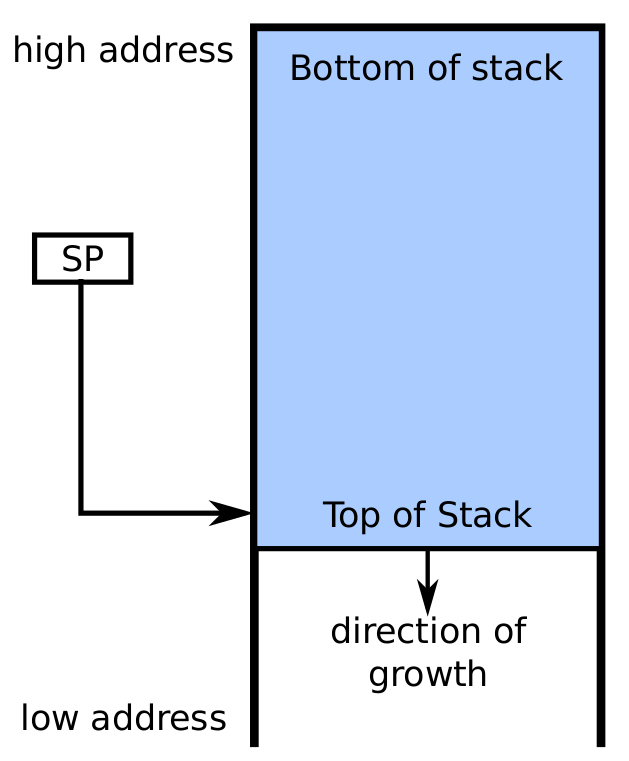
\includegraphics[width=0.2\textwidth]{Stack}\end{figure}

\paragraph{Execution Model --- jump/branch/call commands (x86)}
\begin{itemize}
  \item \code{jmp}: continue execution at operand address
  \item \code{j\$condition}: jump depending on PSW content
  \begin{itemize}
    \item \emph{true} \( \leadsto \) jump
    \item \emph{false} \( \leadsto \) continue
    \item examples: \code{je} (jump equal), \code{jz} (jump zero)
  \end{itemize}
  \item \code{call}: push function to stack and jump to it
  \item \code{return}: return from function (jump to return address)
\end{itemize}

\paragraph{Execution Model --- Application Binary Interface (ABI)}
\begin{itemize}
  \item \textbf{Idea}: standardizes binary interface between programs, modules, OS:
  \begin{itemize}
    \item executable/object file layout
    \item calling conventions
    \item alignment rules
  \end{itemize}
  \item \textbf{calling conventions}: standardize exact way function calls are implemented
  \begin{itemize}
    \item[$ \leadsto $] interoperability between compilers
  \end{itemize}
\end{itemize}

\paragraph{Execution Model --- calling conventions (x86)}
\begin{itemize}
  \item function call --- \textbf{caller}:
  \begin{enumerate}
    \item save local scope state 
    \item set up parameters where function can find them
    \item transfer control flow
  \end{enumerate}
  \item function call --- \textbf{called function}:
  \begin{enumerate}
    \item set up new local scope (local variables)
    \item perform duty
    \item put return value where caller can find it
    \item jump back to caller (IP)
  \end{enumerate}
\end{itemize}

\paragraph{Passing parameters to the system}
\begin{itemize}
  \item parameters are passed through \textbf{system calls}
  \item call number + specific parameters must be passed
  \item parameters can be transferred through
  \begin{itemize}
    \item \textbf{CPU registers} (\textasciitilde 6)
    \item \textbf{Main Memory} (heap/stack -- more parameters, data types)
  \end{itemize}
  \item ABI specifies how to pass parameters
  \item \textbf{return code} needs to be returned to application
  \begin{itemize}
    \item \emph{negative}: error code
    \item \emph{positive + 0}: success
    \item usually returned via A+D registers
  \end{itemize}
\end{itemize}

\paragraph{System call handler}
\begin{itemize}
  \item implements the actual service called through a syscall:
  \begin{enumerate}
    \item saves tainted registers
    \item reads passed parameters
    \item sanitizes/checks parameters
    \item checks if caller has enough permissions to perform the requested action
    \item performs requested action in behalf of the caller
    \item returns to caller with success/error code
  \end{enumerate}
\end{itemize}

\paragraph{Process API --- creation}
\begin{itemize}
  \item process creation events:
  \begin{enumerate}
    \item system initialization
    \item process creation syscall
    \item user requests process creation
    \item batch job-initiation
  \end{enumerate}
  \item events map to two mechanisms:
  \begin{enumerate}
    \item Kernel spawns initial user space process on boot (Linux: \code{init})
    \item User space processes can spawn other processes (within their quota)
  \end{enumerate}
\end{itemize}

\paragraph{Process API --- creation (POSIX)}
\begin{itemize}
  \item \code{PID}: identifies process
  \item \code{pid = fork()}: duplicates current process:
  \begin{itemize}
    \item returns \code{0} to new child
    \item returns new \code{PID} to parent
    \item[$ \leadsto $] child and parent independent after \code{fork}
  \end{itemize}
  \item \code{exec(name)}: replaces own memory based on executable file
  \begin{itemize}
    \item \code{name} specifies binary executable file
  \end{itemize}
  \item \code{exit(status)}: terminates process, returns \code{status}
  \item \code{pid = waitpid(pid, \&status)}: wait for child termination
  \begin{itemize}
    \item \code{pid}: process to wait for
    \item \code{status}: points to data structure that returns information about the process (e.g., exit status)
    \item passed \code{pid} is returned on success, \code{-1} otherwise
  \end{itemize}
  \item \textbf{process tree}: processes create child processes, which create child processes, \dots
  \begin{itemize}
    \item parent and child execute concurrently
    \item parent waits for child to terminate (collecting the exit state)
  \end{itemize}
\end{itemize}

\paragraph{Daemons}
\begin{itemize}
  \item[=] program designed to run in the background
  \item detached from parent process after creation, reattached to process tree root (\code{init})
\end{itemize}

\paragraph{Process States}
\begin{itemize}
  \item \textbf{blocking}: process does nothing but wait \\*
    - usually happens on syscalls (OS doesn't run process until event happens)
\end{itemize}

\begin{figure}[h]\centering\label{ProcessState}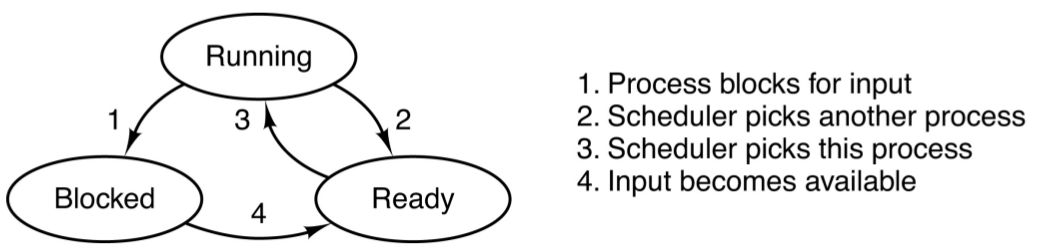
\includegraphics[width=0.4\textwidth]{ProcessState}\end{figure}

\paragraph{Process Termination}
\begin{itemize}
  \item different termination events: 
  \begin{enumerate}
    \item normal exit (voluntary) \\*
      - \code{return 0} at end of \code{main} \\*
      - \code{exit(0)}
    \item error exit (voluntary) \\*
      - \code{return x} (\code{x} \( \neq 0 \)) at end of \code{main} \\*
      - \code{exit(x)} (\code{x} \( \neq 0 \)) \\*
      - \code{abort()}
    \item fatal error (involuntary) \\*
      - OS kills process after exception \\*
      - process exceeds allowed resources
    \item killed by another process (involuntary) \\*
      - another process sends kill signal (only as parent process or administrator)
  \end{enumerate}
\end{itemize}

\paragraph{Exit Status}
\begin{itemize}
  \item voluntary exit: process returns exit status (integer)
  \item resources not completely freed after process terminates
    \( \leadsto \) \textbf{Zombie} or \textbf{process stub} (contains exit status until collected via \code{waitpid})
  \item \textbf{Orphans}: Processes without parents
  \begin{itemize}
    \item usually adopted by \code{init}
    \item some systems kill all children when parent is killed
  \end{itemize}
  \item exit status on involuntary exit:
  \begin{itemize}
    \item Bits \code{0-6}: signal number that killed process (\code{0} on normal exit)
    \item Bit \code{7}: set if process was killed by signal
    \item Bits \code{8-15}: \code{0} if killed by signal (exit status on normal exit)
  \end{itemize}
\end{itemize}
